\section{Unsaturated (Richards) consolidation}

\subsubsection*{Fluid mass and momentum balance}
The general fluid mass balance equation for a multi-phase fluid system is simply an extension of Eq. \ref{eqch14:genmass},

\begin{equation}
\frac{\partial }{\partial t}\left( \phi {{S}_{\alpha }}\rho  \right)+\frac{\partial }{\partial {{x}_{i}}}\left( \phi {{S}_{\alpha }}\rho {{v}_{i}} \right)=Q
\end{equation}

where $S_\alpha$ is saturation of fluid $\alpha $ and $Q$ is the source term. We are interested in a Richards type model for the evolution of fluid pressure under the assumption that the gas phase is immobile, i.e. $v_{gi}=0$. Assuming incompressible grains, $\alpha =0$, and expanding terms as in the single phase case, we obtain the following Richards equation for an unsaturated deformable porous medium,

\begin{eqnarray}
\left( {{S}_{w}}\frac{\phi }{{{K}_{w}}}\frac{d{{p}_{w}}}{dt}-\phi {{\rho }_{w}}\frac{d{{S}_{nw}}}{d{{p}_{c}}} \right)\frac{d{{p}_{w}}}{dt}+\nabla \cdot \left\{ \frac{\mathbf{k}k_{w}^{r}}{{{\mu }_{w}}}\left( -\nabla {{p}_{w}}+{{\rho }_{w}}\mathbf{g} \right) \right\}+\nonumber\\
{{\text{S}}_{w}}{{\rho }_{w}}\nabla \cdot \frac{d\mathbf{u}}{dt}=Q.
\label{eqn:uc2}
\end{eqnarray}

A constitutive equation, the water content function obtained by experiments, characterizes the relationship between $p_c$ and $\sat _w$, and therefore the derivative $dS_w/dp_c$.

\subsubsection*{Solid momentum balance}
The deformation process is described in the same manner as for the single phase case, but now fluid pressure acting on the grains is also dependent on the liquid saturation,

\begin{eqnarray}
\nabla\cdot
(\sigma - S_w p_w \bf I) + \rho g = 0
\label{eqn:mb_us}
\end{eqnarray}

\subsubsection*{FEM solution scheme}
The standard Galerkin finite element approach is applied for the numerical solution of the PDEs (\ref{eqn:uc2}) and (\ref{eqn:mb_us}) resulting into the following system of algebraic equations, here solved as a monolithic system,

\begin{eqnarray}
\left[
\begin{array}{cc}
\mathbf{C}_{pp} & \mathbf{C}_{pu}
\\
\mathbf{0} & \mathbf{0}
\end{array}
\right]
\frac{d}{dt}
\left\{
\begin{array}{l}
\mathbf{p_w}
\\
\mathbf{u}
\end{array}
\right\}
+
\left[
\begin{array}{ll}
\mathbf{K}_{pp} & \mathbf{0}
\\
\mathbf{K}_{up} & \mathbf{K}_{uu}
\end{array}
\right]
%
\left\{
\begin{array}{l}
\mathbf{p_w}
\\
\mathbf{u}
\end{array}
\right\}
=
\left\{
\begin{array}{l}
\mathbf{r}_p
\\
\mathbf{r}_u
\end{array}
\right\}
\nonumber
\\
\end{eqnarray}
%-------------------------------------------------------------------------
%-------------------------------------------------------------------------

\subsection{Heat Pipe problem}
\subsubsection*{Background}
When an unsaturated porous medium subjected to a constant heat flux and the temperature is sufficiently high, water is heated and vaporizes. Vapor flows under its pressure gradient towards the cooler end where it condenses. Vaporization and condensation produce a liquid saturation gradient, creating a capillary pressure gradient inside the porous medium. Condensate flows towards the hot end under the influence of a capillary pressure gradient. This is a heat pipe in an unsaturated porous medium

Udell and Fitch derived the pressure gradient of each phase in two-phase flow with heat transfer. The generalized form of the Darcy's law is used to calculate velocity fields. 
\begin{equation}
\frac{d p^g}{d x} = \frac{\eta q \nu^g}{\mathbf k k_{\mathrm {rg}} H_{\mathrm {vap}}}
\label{eq:HP1}
\end{equation}
\begin{equation}
\frac{d p^l}{d x} =- \frac{\eta q \nu^l}{\mathbf k k_{\mathrm {rl}} H_{\mathrm {vap}}}
\label{eq:HP2}
\end{equation}
where, $\eta$ is the ratio of heat transport caused by convection to the total heat-flux $q$ (see Helming [1997]). $p$ is phase pressure; $\nu^\gamma=\frac{\mu\gamma}{\rho^\gamma}$; $x$ is space coordinate in the x-direction; $\mathbf k$ is intrinsic permeability; $k_{r\gamma}$ is relative permeability and $H_{\mathrm {vap}}$ is latent heat of water. $\gamma$ is the phase superscript and $g, l$ stand for gas and liquid phase, respectively. Gas pressure is the sum of two partial pressure, i.e. $p^g=p^g_a+p^g_w$.

The density of the gas phase is the sum of air and vapor density. Air density is according to ideal gas equation,
\begin{equation}
\rho_{\mathrm {ga}}=\frac{M_a p_a}{RT} 
\label{eq:HP3}
\end{equation}
Energy transport is described by Zhou et al. [1990] as
\begin{equation}
q=-\kappa_{\mathrm {app}}\frac{\partial d T}{d x} + \dot m_{\mathrm {vap}} H_{\mathrm {vap}}
\label{eq:HP4}
\end{equation}
where, $T$ is temperature, $\kappa_{\mathrm {app}}$ is apparent thermal conductivity.

Since capillary pressure is the difference of phase pressure, hence from Eq. 1, the capillary pressure gradient is
\begin{equation}
\frac{d p^c}{d x} = \frac{\eta q}{\mathbf k H_{\mathrm {vap}}}\left[\frac{\nu^g}{k_{\mathrm {rg}}} + \frac{\nu^l}{k_{\mathrm {rl}}}\right]
\label{eq:HP5}
\end{equation}
Brooks-Corey presented a water saturation-capillary pressure relation in the following form
\begin{equation}
S=\left(\frac{Pd}{p^c}\right)^\lambda
\label{eq:HP6}
\end{equation}
By comparing this with Leverett's [1941] non-dimensional form we get $Pd=\sigma_0\left(\frac{n}{\mathbf k}\right)^{0.5}$ and $n$ is medium porosity. $\sigma_0$ is interfacial tension at reference temperature $T_0$. Here, $S$ is scaled as following 
\begin{equation}
S=\frac{S_{\mathrm {w}}-S_{\mathrm {lr}}}{1-S_{\mathrm {lr}}-S_{\mathrm {gr}}}
\label{eq:HP7}
\end{equation}
The constant $S_{\mathrm {lr}}; S_{\mathrm {gr}}$ are residual saturations. And for interfacial tension we have used following correlation given by Olivella and Gens[2000].
\begin{equation}
\sigma( T)={0.3258C^{1.256}} - {0.148C^{2.256}};~~ T\le 633.15 \mathrm K
\label{eq:surface_tension}
\end{equation}
where, $C=1.0-\frac{T}{647.3~K}$

The Brooks-Corey relative permeability relations are 
\begin{equation}
\mathbf k_{\mathrm {rg}}=\left(1-S\right)^2 \left(1-S^{\frac{2+\lambda}{\lambda}}\right);~~~\mathbf k_{rl}=S^{\frac{2+3\lambda}{\lambda}}
\label{eq:HP8}
\end{equation}
Using Eqs. (\ref{eq:HP5}-\ref{eq:HP6}), we can write following forms of saturation gradient.
\begin{equation}
\frac{d S}{d x}=\frac{S^{1.5}}{P_d}\frac{2\eta q}{\mathbf k H_{\mathrm {vap}}}\left[\frac{\nu^g}{k_{\mathrm {rg}}} + \frac{\nu^l}{k_{\mathrm {rl}}}\right]
\label{eq:HP9}
\end{equation}
Now Eq. (\ref{eq:HP9}) is integrated over two-phase zone. Where two-phase zone can be defined by imposing the limits of integration (see Udell [1985]): $S=S_0$ at $x=0$ and $S=S_1$ at $x=L$.

The saturation vapor density $\rho_{\mathrm {sat}}$, depends on temperature, and is estimated by following relation
\begin{equation}
\rho_{\mathrm {sat}}=1.0\times10^{-3}\exp\left(a-\frac{b}{T}\right)
\label{eq:HP10}
\end{equation}
where, the constants $a=19.81$ and $b=4975.9$.

In the porous medium, we must account for a decrease in vapor density due to capillarity. The amount of decrease in vapor density is describe by the Kelvin equation as follows
\begin{equation}
\rho_{\mathrm {gw}}=\rho_{\mathrm {sat}}\exp\left(-\frac{M_{\mathrm w} p^c}{\rho^l RT}\right)
\label{eq:HP11}
\end{equation}
where $M_{\mathrm w}$ is water molecular weight; $\rho^l$ is liquid density and $R$ is universal gas constant. From Eqs. (\ref{eq:HP10}-\ref{eq:HP11}), we get temperature as function of vapor density and capillary pressure as
\begin{equation}
T=\frac{A}{B}
\label{eq:HP12}
\end{equation}
where
\begin{equation*}
 A=b+\frac{M_{\mathrm w} p^c}{\rho^l R}; B=a-3 -\log\left(\rho_{\mathrm {gw}}\right)
 \label{eq:HP20}
\end{equation*}


$\rho_{\mathrm {gw}}$ is changing with temperature which introduces difficulty for the temperature calculation. Hence we need to know temperature gradient, which is possible from Eq. (\ref{eq:HP12}) along with the vapor pressure gradient 
\begin{equation}
\frac{d p_{\mathrm{gw}}}{d x} = \frac{\eta q \nu^g_w}{\mathbf k k_{\mathrm {rg}} H_{\mathrm {vap}}}
\label{eq:HP18}
\end{equation}
Form of the temperature gradient
\begin{equation}
\frac{d T}{d x}=\frac{\frac{B M_{\mathrm w}}{\rho^l R} \frac{d p^c}{d x} + \frac{A}{p_{\mathrm{gw}}} \frac{d p_{\mathrm{gw}}}{d x}}{B^2+\frac{A}{T}}
\label{eq:HP13}
\end{equation}
Apparent thermal conductivity can be obtained from heat flux divided by temperature gradient (see Udell [1985].


The coupled differential Eqs. (\ref{eq:HP1}), (\ref{eq:HP5}), (\ref{eq:HP9}) and (\ref{eq:HP13} ) are integrated using an Euler method with the following boundary conditions at $x=0$:
\begin{equation}
S=S_0;~~~ p^g=p^g_0;~~~p^c=p^c_0;~~~T=T_0
\label{eq:HP14}
\end{equation}
Material parameters are presented in Table \ref{tab:HP1}.

\subsubsection*{Definition}
The test benchmark problem for heat pipe effects is formulated in one-dimension. 
A horizontal column of length $2.6$~m is filled with fluid subjected to a constant heat flux at the right end where left end temperature maintained below to the saturation temperature.
\begin{figure}[htb]
\begin{center}
\includegraphics[height=1.25cm]{chapter_14/figures/Geo.eps}
\end{center}
\caption{Schematic of the benchmark.}
\label{Fig:HP1}
\end{figure}


\subsubsection*{Results}
In order to establish non-isothermal two-phase flow in the OpenGeoSys, we have verified numerical solutions with analytical results. Profile of water saturation $S_{\mathrm w}$, gas phase pressure $p^g$, liquid phase pressure $p^l$ and temperature $T$ are presented in Figs. \ref{Fig:HP2}, and \ref{Fig:HP4}. Numerical solutions are agreeable. Line elements have been used with variable time steps and a non uniform space discretization.
\begin{figure}[thbp]
\centerline{
\includegraphics[height=3.0in,width=3.0in]{chapter_14/figures/S-Pc.eps}
\includegraphics[height=3.0in,width=3.0in]{chapter_14/figures/Pw-Pg.eps}}
\caption{Comparison of water saturation and pressure profiles from present solution with analytical solution.}
\label{Fig:HP2}
\end{figure}
A finite element approach has been developed for the nonisothermal two-phase flow model based on the $ppT$ formulation. We used a combined monolithic/ staggered coupling scheme i.e. monolithic for the two-phase flow and staggered for the heat transport.
\begin{figure}[htb]
\begin{center}
\includegraphics[height=8cm]{chapter_14/figures/Tg.eps}
\end{center}
\caption{Comparison of temperature profile from present solution with analytical solution.}
\label{Fig:HP4}
\end{figure}
\begin{table}[htbp]
\caption{Material parameters for the heat pipe problem.}
\label{tab:HP1}
\begin{tabular}{l*{4}{l}r}
\hline
\textbf{Meaning} & \textbf{Symbol} &  \textbf{Value} &  \textbf{Unit} \\
\hline
Column length & $L$ & $\mathrm m$ & $2.6$  \\
Liquid dynamic viscosity &  $\mu^l$ & $\mathrm {Pa.s}$ & $1.0\times10^{-3}$ \\
Gas dynamic viscosity & $\mu^g$ & $\mathrm {Pa.s}$ & $1.0\times10^{-5}$ \\
Liquid density &  $\rho^l$ &$\mathrm {kg.m^{-3}}$ & $1.0\times10^{3}$ \\
Permeability & $\mathbf k$ & $ \mathrm {m^2}$ & $1.0\times 10^{-13}$ \\
Porosity & $n$ & $--$ & $0.3$ \\
Residual saturation of water &  $S_{\mathrm{rl}}$ & $--$ & $0.2$ \\
Residual saturation of oil &  $S_{\mathrm{rg}}$ & $--$ & $0$ \\
Soil distribution index &  $\lambda$ & $--$ & $2.0$ \\
Capillary pressure & $p^c(S)$ & $\mathrm {Pa}$ & Brooks-Corey model\\
Relative permeability & $\kappa_{\mathrm {r\gamma}}(S)$ & $--$ & Brooks-Corey model \\ \hline
\end{tabular}
\end{table}

\subsection{DECOVALEX unsaturated test case}
DECOVALEX is an international code comparison project for the verification of thermo-hydro-mechanical (THM) and thermo-hydro-chemical (THC) numerical simulators \cite{BirEtAl:2008}.

\subsubsection*{Definition}
The original DECOVALEX-THM benchmark definition is a 2-D problem \cite{BirEtAl:2008}. For the comparison of different HM swelling models, we consider a simplified case representing a horizontal cross-section through the 2-D domain. Examined here is the isothermal HM consolidation problem with unsaturated flow.

\begin{figure}[!t]
\begin{center}
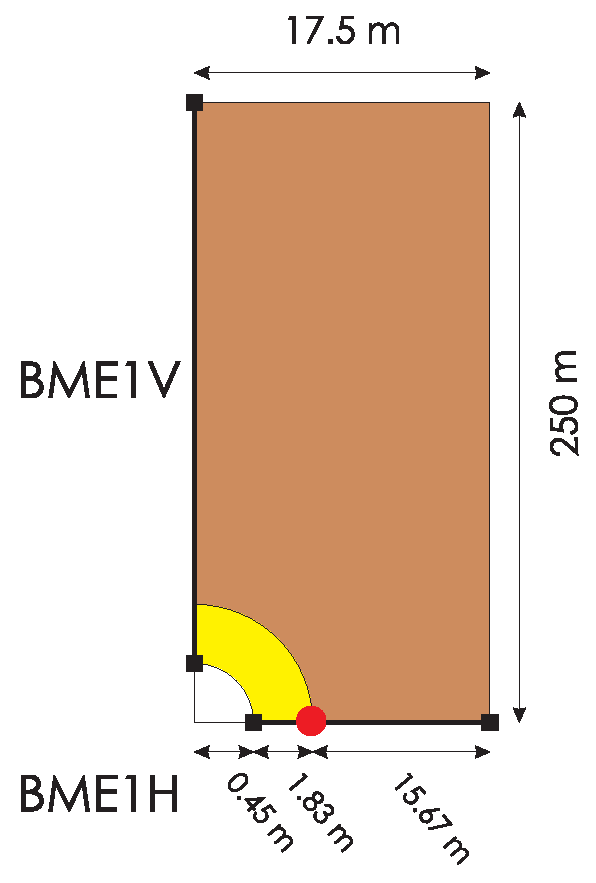
\includegraphics[width=0.3\textwidth]{chapter_14/figures/fig_14_2_15}
\end{center}
\caption{2D DECOVALEX HM definition and simplification for the benchmark exercise BME1H.}
\label{fig:thm-1D}
\end{figure}

\begin{figure}[!t]
\begin{center}
\includegraphics[width=1.0\textwidth]{chapter_14/figures/fig_14_2_16}
\end{center}
\caption{Mesh of the simplified BME1H model including canister, bentonite, and rock mass sections.}
\label{fig:thm-1Dmesh}
\end{figure}

The simplified model takes a rectangle shape. The mesh of the domain together with material types are shown in Fig. \ref{fig:thm-1Dmesh}. Fig. \ref{fig:BME1H} illustrates the definition of initial and boundary conditions for the horizontal cross-section. Observation points are set at $x=0.45\,m, \,x=1.10\,m$ to record temporal breakthrough curves. Material parameters for the rock mass and bentonite are given in Table \ref{tab:hm_rock}.

\begin{table}[!thb]
\begin{center}
\begin{tabular}{lll}
\hline
Parameter   &  Unit  & Value\\
\hline
\textit{Rock mass properties} & & \\
Density &  $kg/m3$ &  2700 \\
Young's modulus &  $GPa$ &  $35$ \\
Poisson ratio & - &  0.3 \\
Porosity & - &  0.01 \\
Saturated permeability &  $m2$  & $1.0\times10^{-17}$ \\
\\
\textit{Bentonite properties} & & \\
Density &  $kg/m3$ &  1600 \\
Young's modulus &  $MPa$ &  $317$\\
Poisson ratio & - &  0.35 \\
Saturated permeability &  $m2$  & $2.0
\times10^{-21}$ \\
\hline
\end{tabular}
\end{center}
\caption{\label{tab:hm_rock}Solid properties of different materials.}
\end{table}

\begin{figure}[!htb]
\begin{center}
%\footnotesize
\scalebox{0.8} % Change this value to rescale the drawing.
{
\begin{pspicture}(0,-1.900625)(18.579687,1.900625)
\definecolor{color7g}{rgb}{1.0,0.0,0.2}
\definecolor{color0g}{rgb}{0.4,0.4,0.4}
\definecolor{color0f}{rgb}{0.6,0.6,0.6}
\psframe[linewidth=0.04,dimen=outer,fillstyle=gradient,gradlines=2000,gradbegin=color0g,gradend=color0f,gradmidpoint=1.0](12.799687,1.0171875)(1.7796875,-1.1428125)
\psframe[linewidth=0.04,dimen=outer,fillstyle=gradient,gradlines=2000,gradbegin=color7g,gradend=color7g,gradmidpoint=1.0](3.7996874,1.0171875)(1.7596875,-1.1228125)
\psframe[linewidth=0.04,dimen=outer,fillstyle=gradient,gradlines=2000,gradbegin=blue,gradend=blue,gradmidpoint=1.0](6.4396877,1.0171875)(3.7796874,-1.1428125)
\psframe[linewidth=0.04,dimen=outer](18.539688,1.4571875)(18.519688,1.2971874)
\usefont{T1}{ptm}{m}{n}
\rput(7.403125,1.5271875){$u_y$=0, $\sigma_{xy}$=0}
\usefont{T1}{ptm}{m}{n}
\rput(7.383125,-1.6728125){$u_y$=0, $\sigma_{xy}=0$}
\usefont{T1}{ptm}{m}{n}
\rput(14,0.2471875){$u_x=0, \sigma_{xy}=0$}
\usefont{T1}{ptm}{m}{n}
\rput(13.8,-0.1){$p^l=10^6$Pa}
\usefont{T1}{ptm}{m}{n}
\rput(0.973125,0.2471875){$u_x$=0}
\usefont{T1}{ptm}{m}{n}
\rput(0.99,-0.1){$\sigma_{xy}$=0}
\usefont{T1}{ptm}{m}{n}
\rput(5.,0.24){\color{red}S0=0.65}
\usefont{T1}{ptm}{m}{n}
\rput(5.1,-0.1){\color{yellow}($p^l=-7\times10^7$Pa)}
\usefont{T1}{ptm}{m}{n}
\rput(9,-0.1728125){\color{yellow}$p^l=10^5$Pa}
\end{pspicture}
}
\end{center}
\caption{Simplified horizontal cross-section model.}
\label{fig:BME1H}
\end{figure}

The dependency of capillary pressure and relative permeability on liquid saturation for both rock and bentonite are depicted in Fig. \ref{fig:cp_cp}.

\begin{figure}[!htb]
\begin{center}
\includegraphics[width=0.49\textwidth]{chapter_14/figures/fig_14_2_18_a}
\includegraphics[width=0.49\textwidth]{chapter_14/figures/fig_14_2_18_b}
\end{center}
\caption{Capillary pressure and relative permeability functions.}
\label{fig:cp_cp}
\end{figure}

\begin{figure}[!t]
\begin{center}
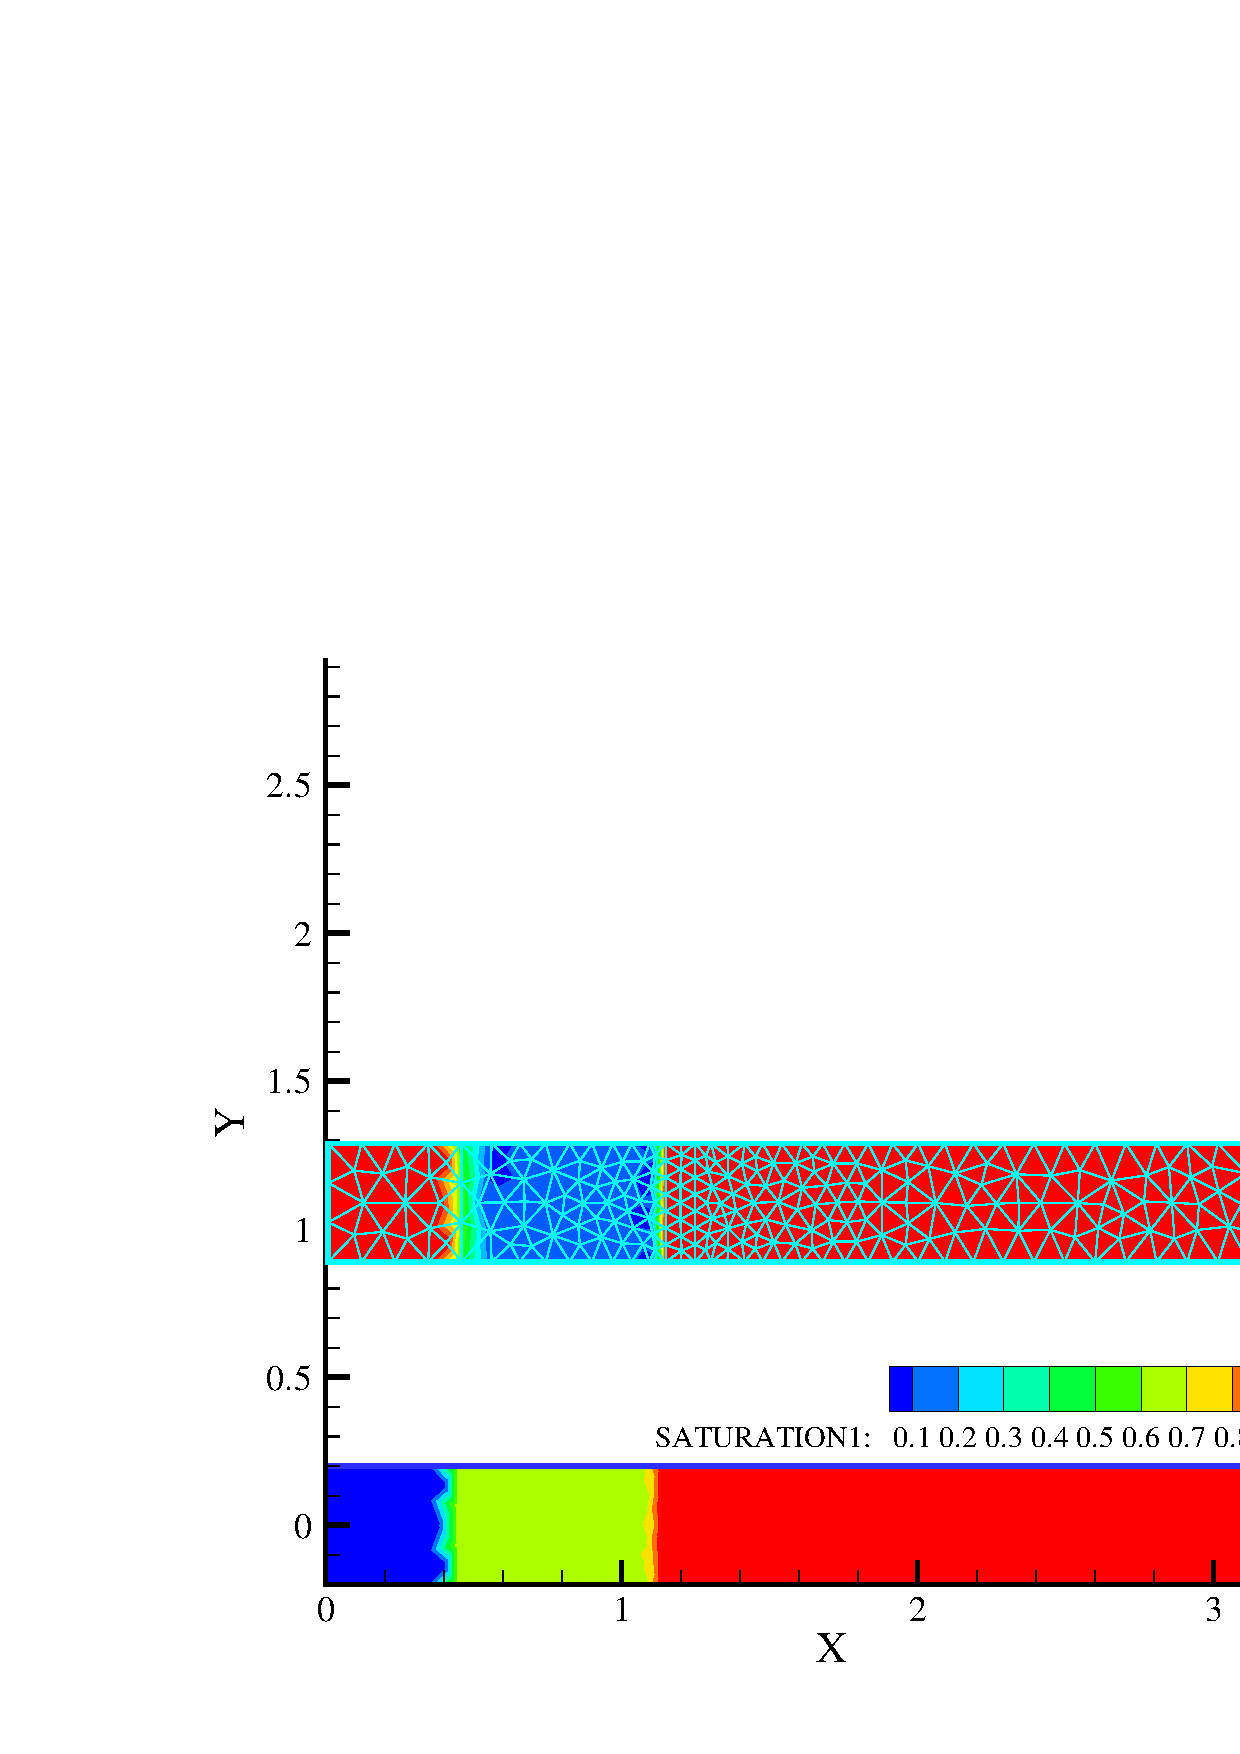
\includegraphics[width=0.7\textwidth]{chapter_14/figures/fig_14_2_19}
\end{center}
\caption{Distribution of saturation and vertical swelling stress}
\label{fig:hmswl_cont}
%\end{figure}
%\begin{figure}[!t]
\begin{center}
\includegraphics[width=0.49\textwidth]{chapter_14/figures/fig_14_2_20_a}
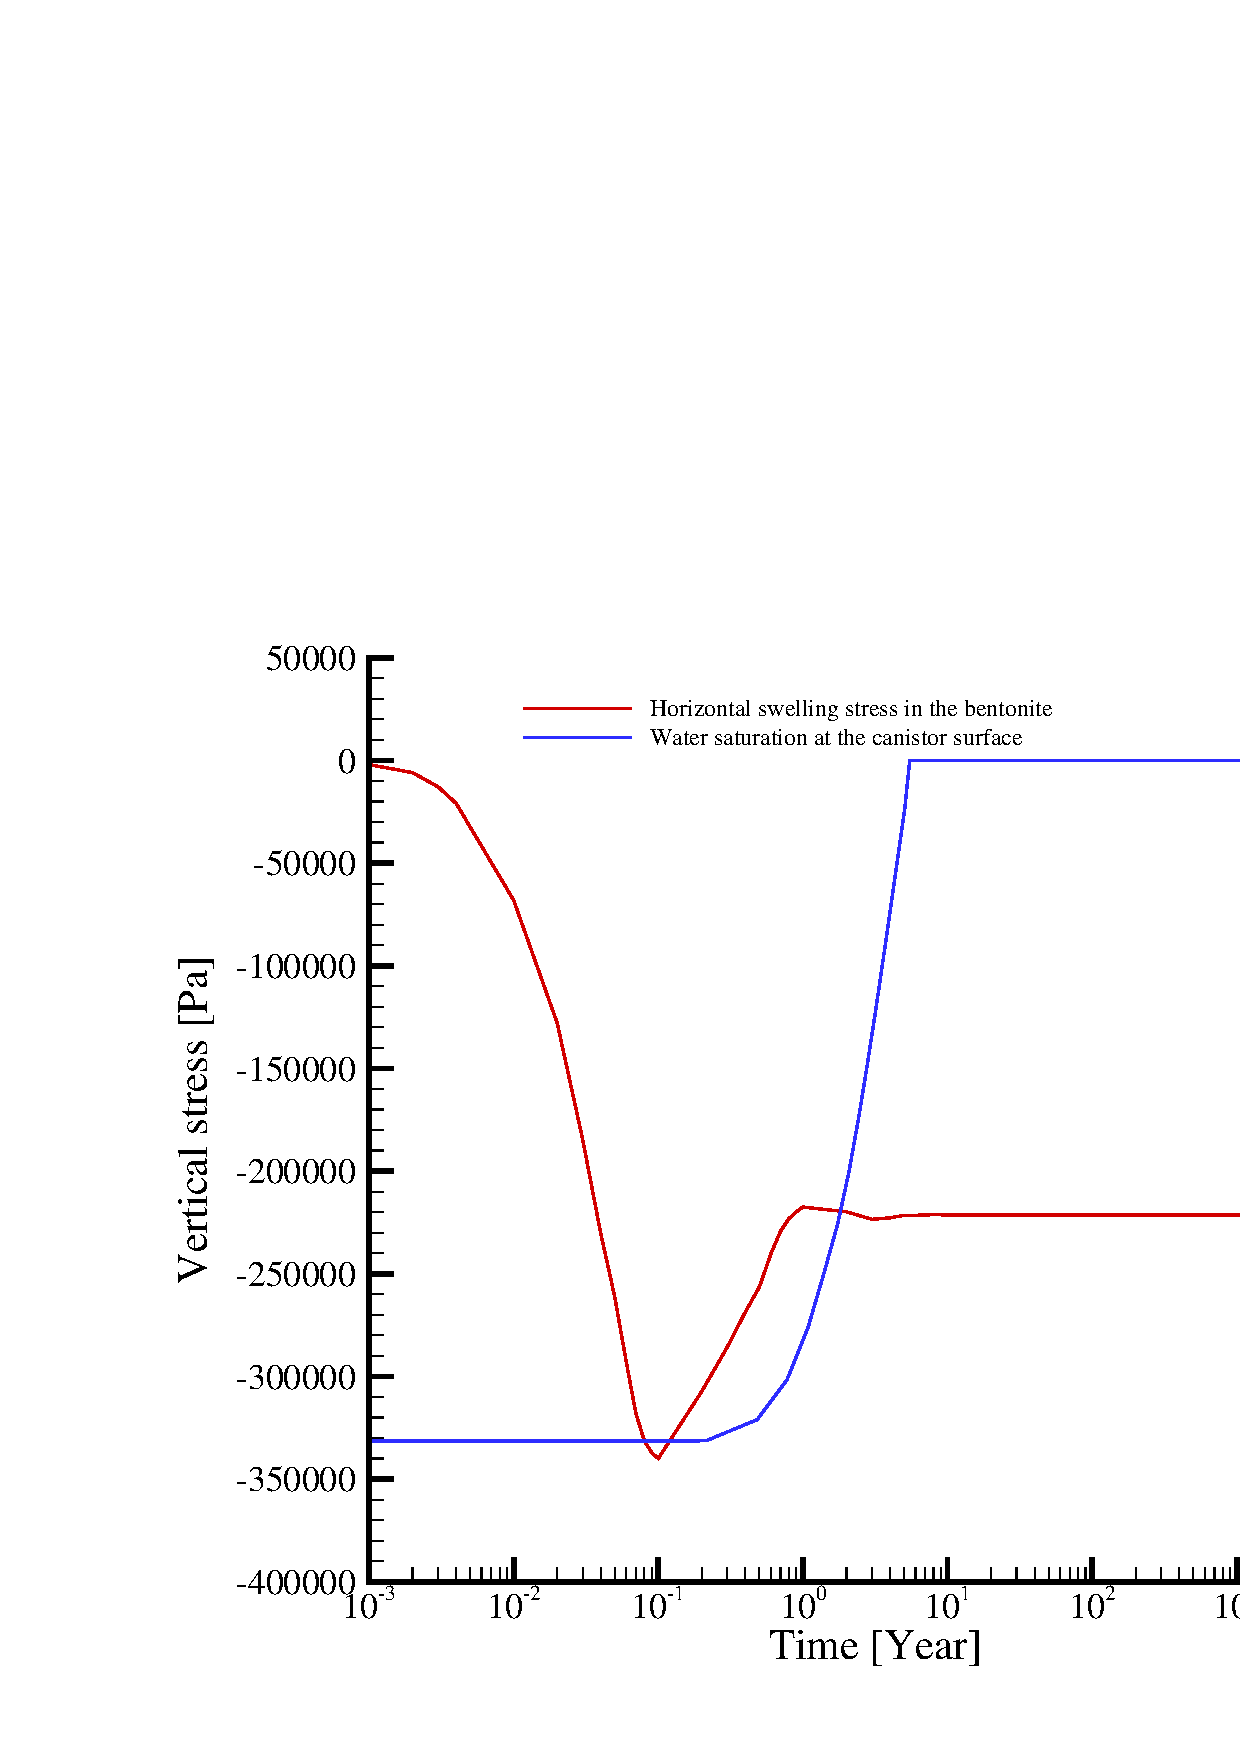
\includegraphics[width=0.49\textwidth]{chapter_14/figures/fig_14_2_20_b}
\end{center}
\caption{Horizontal profile (top) and temporal evolution at observation point (bottom) of water saturation and swelling stress}
\label{fig:deco-hm}
\end{figure}

\subsubsection*{Results}
Fig. \ref{fig:hmswl_cont} displays a contour plot of saturation and vertical swelling stress in the domain. Swelling stress in the bentonite is clearly induced by change of water saturation. Fig. \ref{fig:deco-hm} shows the simulated horizontal profiles (top) and temporal evolutions at the observation point (bottom) of water saturation and swelling stress based on the linear swelling model proposed by Rutqvist (2005) \cite{Jonny05}, which defines the increment of swelling stress to be proportional to liquid saturation increment,

\begin{equation}
\Delta \sigma ^{sw}=\beta \Delta S_w,
\end{equation}

where $\beta $ is a swelling coefficient that could be called the maximum swelling stress. As the saturation change approaches unity, swelling stress approaches $\beta $.

Fig. \ref{fig:deco-hm} shows the simulated horizontal profiles and temporal evolutions at the observation point of water saturation and swelling stress based on the linear swelling model proposed by Rutqvist (2005) \cite{Jonny05}.
